%%%%%%%%%%%%%%%%%%%%%%%%%%%%%%%%%%%%%%%%%
% Thin Sectioned Essay
% LaTeX Template
% Version 1.0 (3/8/13)
%
% This template has been downloaded from:
% http://www.LaTeXTemplates.com
%
% Original Author:
% Nicolas Diaz (nsdiaz@uc.cl) with extensive modifications by:
% Vel (vel@latextemplates.com)
%
% License:
% CC BY-NC-SA 3.0 (http://creativecommons.org/licenses/by-nc-sa/3.0/)
%
%%%%%%%%%%%%%%%%%%%%%%%%%%%%%%%%%%%%%%%%%

%----------------------------------------------------------------------------------------
%	PACKAGES AND OTHER DOCUMENT CONFIGURATIONS
%----------------------------------------------------------------------------------------

\documentclass[a4paper, 12pt]{article} % Font size (can be 10pt, 11pt or 12pt) and paper size (remove a4paper for US letter paper)
\usepackage[top=1in, bottom=1.25in, left=1in, right=1in]{geometry}
\usepackage[protrusion=true,expansion=true]{microtype} % Better typography
\usepackage{graphicx} % Required for including pictures
\usepackage{wrapfig} % Allows in-line images
\usepackage{caption}
\usepackage{amsmath}
\usepackage{mathtools}
\usepackage{float}
\usepackage{hyperref}
\usepackage{mathpazo} % Use the Palatino font
\usepackage[T1]{fontenc} % Required for accented characters
\usepackage{cancel}
\usepackage{natbib}
\linespread{1.05} % Change line spacing here, Palatino benefits from a slight increase by default

\makeatletter
\renewcommand\@biblabel[1]{\textbf{#1.}} % Change the square brackets for each bibliography item from '[1]' to '1.'
\renewcommand{\@listI}{\itemsep=0pt} % Reduce the space between items in the itemize and enumerate environments and the bibliography

\renewcommand{\maketitle}{ % Customize the title - do not edit title and author name here, see the TITLE block below
\begin{flushright} % Right align
{\LARGE\@title} % Increase the font size of the title

\vspace{50pt} % Some vertical space between the title and author name

{\large\@author} % Author name
\\\@date % Date

\vspace{40pt} % Some vertical space between the author block and abstract
\end{flushright}
}

%----------------------------------------------------------------------------------------
%	TITLE
%----------------------------------------------------------------------------------------

\title{\textbf{Modelling the Milky Way Galaxy \& the Large Magellanic Cloud}} % Subtitle

%\author{\textsc{Juan Nicol\'as Garavito Camargo } % Author
%\\{\textit{Departamento de F\'isica\\}
%\textit{Universidad de los Andes, Bogot\'a, Colombia}}} % Institution

\date{August, 2015} % Date

%----------------------------------------------------------------------------------------
\begin{document}

\maketitle


\section{Useful Quantities and definitions}

In this section some common quantities useful for describe the density profiles
are defined and explained.


\subsection{Critical density of the Universe:}

The Critial density of the universe is defined as:

\begin{equation}
\rho_c = \dfrac{3H^2}{8 \pi G}
\end{equation}

Where $H$ is the Hubble parameter and this parameter depends on the cosmological parameters.
This density ... 

\subsection{Virialization}

A dark matter halo is virialized when it is in equilibrium, such
an equilibrium occurs after the dark matter have collapsed and
the force of gravity equals the \textbf{relaxation} processes
\cite{BinneyTremaine08}. This happens when the dark matter
reach an overdensity value $\Delta_{vir}$. This overdensity corresponds
to a radius and a mass $r_{vir}$ \& $M_{vir}$ respectively. 

 $\Delta_{vir} = \frac{\rho_{vir}}{\rho_c}$.
For a cosmolgy with ($\Omega_m + \Omega_{\Lambda} = 1$) the
solution for the \textbf{Top Hat} model can be  approximated by:

\begin{equation}
\Delta_{vir} = (18 \pi^2 + 82x - 39x^2)/\Omega(z) 
\end{equation}

\cite{EkeColeFrenk96,BryanNorman98} Where $x=\Omega(z)-1$.
For the present time ($z=0$)  $\Delta_{vir}=360$.

The behavior of this function is shown in Fig.\ref{fig:dvir}

\begin{figure}[H]\label{fig:dvir}
\centering
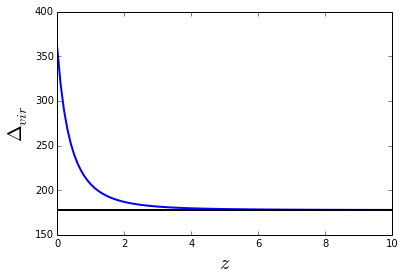
\includegraphics[scale=0.5]{deltavir.png}
\caption{The solid blue line shows the behaviour of $\Delta_{vir}$ 
as function of the redshift. The black line show the value of 
$\Delta_{vir}=173$ at $z>4$}
\end{figure}

The virial density now can be expressed in terms of $\Delta_{vir}$: 

\begin{equation}\label{eq:rhovir}
\rho_{vir} = \frac{3M_{vir}}{4 \pi r_{vir}^3} = \Delta_{vir} \Omega_m \rho_{crit} 
\end{equation}

Where $\Omega_m$ is the density parameter that give as the abundance of matter in the 
Universe, it is define as $\Omega_m = \rho / rho_c$ and the actual value is $\Omega_m \simeq 0.3$  
Once the virial density is defined with \ref{eq:rhovir} for a given $z$ then the radius 
and the virial mass can be related:

\begin{equation}
r_{vir} = \left( \frac{3M_{vir}}{4 \pi \Delta_{vir} \Omega_m \rho_{crit} } \right )^{1/3}
\end{equation}

For example for a halo of mass $M = 1 \times 10^{12}M_{\odot}$ the corresponding radius 
is $r_{vir}=262.4$ Kpc

\subsection{$r_{200}$ \& $M_{200}$}

There is another radious and mass of particular interest. This is the radius that enclosed a density
of 200 times the density of the Universe. $M_{200}$ is defined as:  

\begin{equation}\label{eq:m200}
M_{200} = 200 \rho_c \dfrac{4}{3} \pi r_{200}^3
\end{equation}

In the same way $M_{vir}$ is defined as:

\begin{equation}\label{eq:mvir}
M_{vir} = \Delta_{vir} \Omega_m \rho_c \dfrac{4}{3} \pi r_{vir}^3
\end{equation}

The critial density $rho_c$ is the same for both cases, then it is possible
to relate both masses from Eq\ref{eq:m200} and Eq\ref{eq:mvir} as follows:

\begin{equation}
\dfrac{M_{200}}{M_{vir}} = \left(  \dfrac{200}{ \Delta_{vir} \Omega_m}  \right) \left( \dfrac{r_{200}}{r_{vir}}  \right)^3
\end{equation}

Here is common to call $q = \left(  \dfrac{200}{ \Delta_{vir} \Omega_m}  \right) $,  at $z=0$ $q=2.053$.

\begin{equation}\label{eq:q}
\dfrac{M_{200}}{M_{vir}} = q \left( \dfrac{r_{200}}{r_{vir}}  \right)^3
\end{equation}

This Eq.\ref{eq:q} relates $M_{vir}$ and $M_{200}$ for a given $r{vir}$ and $r_{200}$. 

\section{Densities profiles}

\subsection{Plummer}

The plumer density profile is one of the simplest models which describes
a constant density near the center and falls at large radius.

\begin{equation}
\Phi_P(r) = - \frac{GM}{\sqrt{r^2+a^2}}
\end{equation}


Where $a$ is call the scale length. The scale length set the length $a$ in which the mayority of the density is enclosed. Note
that if $a$ is cero the plummer potential would be exactly as the potential of a point mass.
In the other hand if $a$ goes to infty the potential is rewpresenting a very extended mass source.
In other words the scale length set up the size of the volume in which the mass $M$ is enclosed.


\begin{figure}[H]
\centering
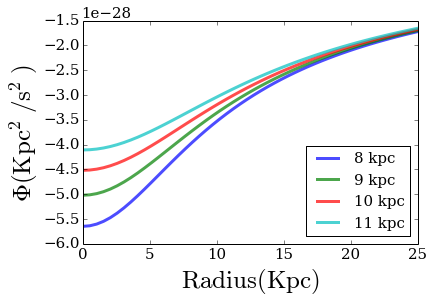
\includegraphics[scale=0.5]{plummer_phi.png}
\end{figure}


\begin{equation}
\nabla ^2 \Phi_P(r) = 4 \pi G \rho_P(r) = \frac{1}{r^2}\frac{d}{dr} \left (  r^2 \frac{d\Phi_P(r)}{dr} \right)
\end{equation}

\begin{equation}
\rho_P (r) = \frac{3M}{4\pi a^3} (1 + \frac{r^2}{a^2})^{-5/2}
\end{equation}


\begin{figure}[H]
\centering
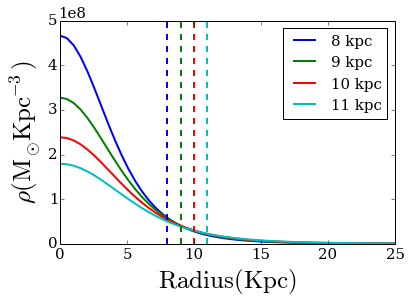
\includegraphics[scale=0.5]{plummer_density.png}
\end{figure}



The enclosed mass can be derived from the density by integrating over the volume.

\begin{equation}
M_P(<r) = 4 \pi \int_0^r r'^2\frac{3M}{4\pi a^3} (1 + \frac{r'^2}{a^2})^{-5/2} dr' = \frac{3M}{a^3} \left( \frac{a^4 r^3 \sqrt{r^2/a^2 + 1}}{3(r^2 + a^2)^2}  \right)
\end{equation}

\begin{equation}
M_P(<r) = M \frac{r^3}{(a^2+r^2)^{3/2}}
\end{equation}


\begin{figure}[H]
\centering
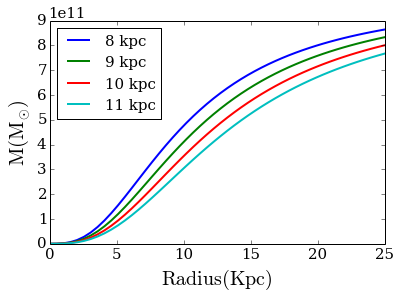
\includegraphics[scale=0.5]{plummer_mass.png}
\end{figure}


\begin{equation}
F_g = \frac{GmM}{r^2} = ma_c = m \frac{v_c^2}{r}
\end{equation}

\begin{equation}
v_c = \sqrt{\frac{GM(<r)}{r}}
\end{equation}

\begin{equation}
v_c = \sqrt{GM(\frac{r^2}{(r^2+a^2)^{3/2}})}
\end{equation}


\begin{figure}[H]
\centering
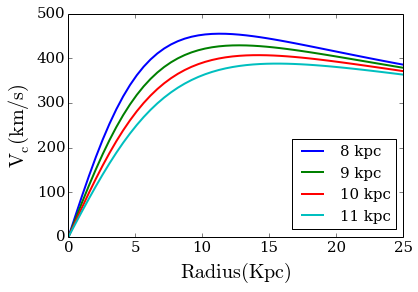
\includegraphics[scale=0.5]{plummer_velocity.png}
\end{figure}



\subsection{Hernquist profile}

The Hernquist profile is derived in such a way that it follows the 

\begin{equation}
\rho_{Hernquist}(r) =  \frac{M}{2\pi} \frac{a}{r(r+a)^3}
\end{equation}

\begin{equation}
M_{Hernquist}(<r) = 2aM \int \frac{r}{(r+a)^3}dr
\end{equation}

\begin{equation}
M_{Hernquist}(<r) = M \frac{r^2}{(r+a)^2}
\end{equation}

\begin{equation}
\Phi = - \frac{GM}{r+a}
\end{equation}

\begin{equation}
v_c(r) = GM \frac{r}{(r+a)^2}
\end{equation}

\begin{figure}[H]
\centering
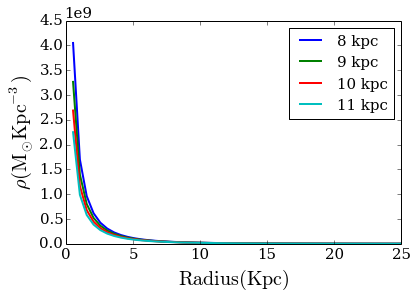
\includegraphics[scale=0.7]{hern_density.png}
\end{figure}

\begin{figure}[H]
\centering
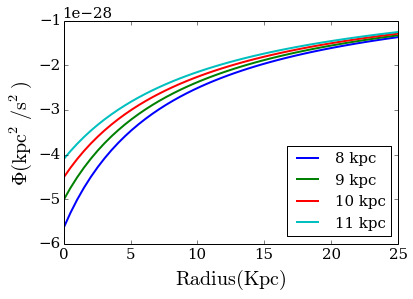
\includegraphics[scale=0.7]{hern_potential.png}
\end{figure}

\begin{figure}[H]
\centering
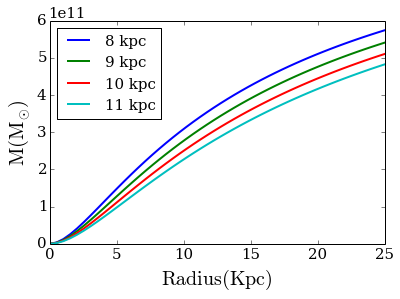
\includegraphics[scale=0.7]{hern_mass.png}
\end{figure}

\begin{figure}[H]
\centering
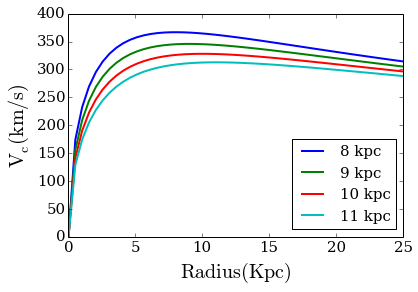
\includegraphics[scale=0.7]{hern_velocity.png}
\end{figure}


\subsection{Singular Isothermal Sphere}

The Singular Isothermal Sphere (\textbf{SIS}) describes a system in which the particles follow
a Maxwellian density distribution. With this distribution and the Poisson equation the follow
density profiles could be derived.


\begin{equation}
\rho_{iso}(r) = \dfrac{\sigma ^2}{2\pi G r^2}
\end{equation}

Following the same procedure as with the previuos profiles we find $M, \Phi$  and $v_c$.

\begin{equation}
M_{iso}(<r) = \dfrac{2 \sigma r}{G}
\end{equation}

\begin{equation}
\Phi_{iso}(r) = 2 \sigma^2 ln(r)  + const.
\end{equation}

\begin{equation}\label{eq:SISv}
v_c(r) = \sqrt{2}\sigma
\end{equation}

This profile is quite different to the previous ones due to the fact that here the input is
the velocity instead of the total Mass.

\begin{figure}[H]
\centering
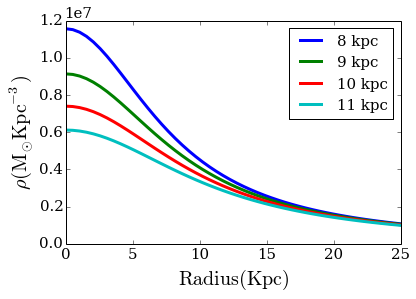
\includegraphics[scale=0.7]{sis_density.png}
\end{figure} 

\begin{figure}[H]
\centering
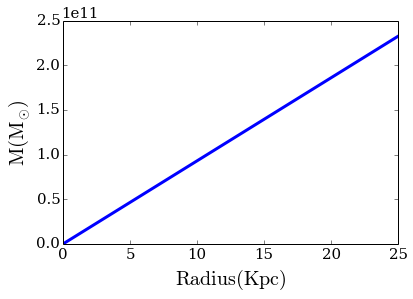
\includegraphics[scale=0.7]{sis_mass.png}
\end{figure}

\begin{figure}[H]
\centering
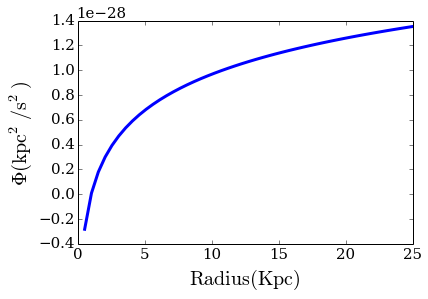
\includegraphics[scale=0.7]{sis_phi.png}
\end{figure}


\subsection{NFW}


\begin{equation}\label{eq:rhoNFW}
\rho_{NFW}(r) = \dfrac{M}{2\pi a^3(r/a) (1 + r/a)^2}
\end{equation}


\begin{equation}\label{eq:MNFW}
M_{NFW}(r) =  M  \left(  ln(1 + x) - \frac{x}{1 + x} \right)
\end{equation}

Where $x = r/a$, is useful to define the function $f(x)$ as:

\begin{equation}
f(x) = ln(1 + x) - \frac{x}{1 + x} 
\end{equation}

Then \ref{eq:MNFW} can be expresed as:

\begin{equation}\label{eq:M2NFW}
M_{NFW} = 4 \pi \rho_a a^3 f(x)
\end{equation}

\begin{equation}\label{PhiNFW}
\Phi_{NFW} = -4\pi G M \frac{ln(1 + r/a)}{r}
\end{equation}

\begin{equation}\label{eq:cnfwz0}
c(M_{vir}) = 9.60  \left( \frac{M_{vir}}{10^{12}h^{-1}M_{\odot}} \right)^{-0.075}
\end{equation}



\begin{equation}\label{vcNFW}
v_c(r) = \sqrt{\left(\dfrac{M(r)G}{r}\right)} = \sqrt{\left( \dfrac{2 M  \left(  ln(1 + c) - \frac{c}{1 + c} \right)}{r} \right)}
\end{equation}


\begin{figure}[H]
\centering
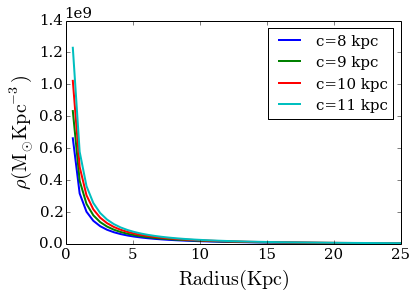
\includegraphics[scale=0.7]{NFW_density.png}
\end{figure}

\begin{figure}[H]
\centering
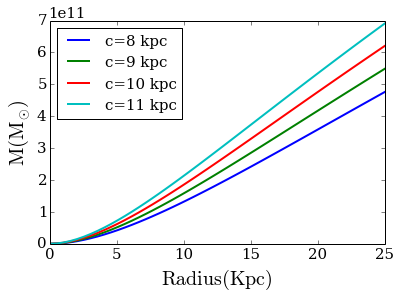
\includegraphics[scale=0.7]{NFW_mass.png}
\end{figure}

\begin{figure}[H]
\centering
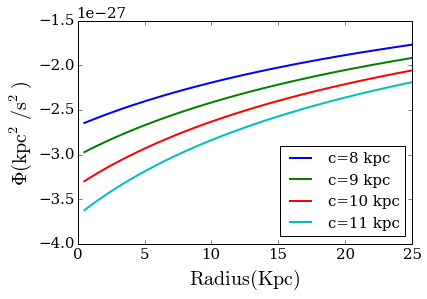
\includegraphics[scale=0.7]{NFW_potential.png}
\end{figure}

\begin{figure}[H]
\centering
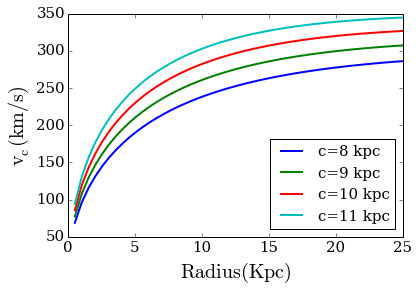
\includegraphics[scale=0.7]{NFW_vc.png}
\end{figure}



\section{Conversion from NFW to the Hernquist profile}

The average density of the NFW distribution can be expressed as:

\begin{equation}
\bar \rho_{NFW}(r) = \dfrac{3M_{NFW}(r)}{4 \pi r^3} 
\end{equation}

And with eq.\ref{eq:M2NFW} the $\bar{\rho_{NFW}(r)}$ takes de form:

\begin{equation}
\bar \rho_{NFW}(r) = 3 \rho_a \left( \dfrac{a}{r} \right)^{3}  f(x)
\end{equation}

Now if we want to find the relationship betwee $r_{200}$ and $r_{vir}$ 
for the NFW profile we have to apply eq\ref{eq:q}. 

\begin{equation}
q = \dfrac{3 \rho_a \dfrac{a}{r_{200}} f(c_{200})}{3 \rho_a \dfrac{a}{r_{vir}}f(c)} = \dfrac{c_{200}^{3}f(c_{200})}{c_{vir^3}f(c_{vir})}
\end{equation}


\begin{equation}\label{eq:c200cvir}
\dfrac{c_{200}}{c_{vir}} = \left( \dfrac{f(c_{200})}{qf(c_{vir})} \right)^{1/3}
\end{equation}

For $c_{vir} = 10$ this function is shown in Fig.\ref{fig:c200cvir}, where 
$y = \dfrac{c_{200}}{c_{vir}} - \left( \dfrac{f(c_{200})}{qf(c_{vir})} \right)^{1/3}$

\begin{figure}[H]\label{fig:c200cvir}
\centering
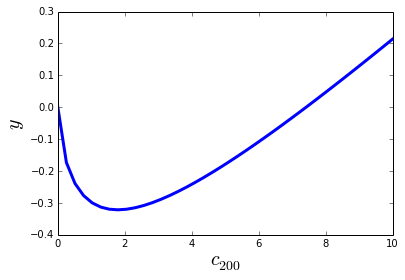
\includegraphics[scale=0.7]{c200cvir.png}
\end{figure}

Note that the solution of Eq.\ref{eq:c200cvir} is when $y=0$, one 
solution is $c_{200}=0$ but this is not of particular interest for us. 

The other solution is computed analytically using the bisection algorithm.
$c_{200} = 7.4$

In order to seek the equivalence between the NFW and the Hernquist profile, 
We have to match the same enclosed mass of both profiles at a given radius.
To his end we have to find $M_H$ in terms of $r_s$. 

\begin{equation}
M_H(r) = M_{NFW}(r)
\end{equation}

\begin{equation}
\frac{M_H r^2}{a^2 + r^2} = 4 \pi \rho_s r_s^3 \left[ Ln(1 + x) - \frac{x}{1+x}  \right]
\end{equation}

In the limit $r \rightarrow 0$ 

\begin{equation}
M_H = \dfrac{4 \pi \rho_s r_s^3 a^2}{r^2} \left[ (x - \dfrac{x^2}{2}) - x  \right]
\end{equation}

\begin{equation}
M_H = 4 \pi \rho_s r_s^3 \dfrac{a^2}{r^2} \left(  - \dfrac{r^2}{2r_s^2} \right)
\end{equation}

\begin{equation}
M_H = 2 \pi r_s a^2
\end{equation}
 
With this relation is possible now to match both profiles at a given radius $\tilde{r}$ 

\begin{equation}
M_H(\tilde{r}) = M_{NFW}(\tilde{r}) 
\end{equation}

\begin{equation}
2 \pi \rho_s a^2 r_s \dfrac{\tilde{r}^2}{a^2} \dfrac{1}{\left( 1 + \dfrac{\tilde{r}}{a}\right)^2} = 4 \pi \rho_s r_s^3 \left( Ln \left(1 + \dfrac{\tilde{r}}{r_s} \right)  - \dfrac{\tilde{r}}{\tilde{r} + r_s} \right)
\end{equation}

\begin{equation}
\dfrac{\tilde{r}^2 a^2}{(a + \tilde{r})^2} = 2 r_s^2 \left( Ln \left (1 +  \dfrac{\tilde{r}}{r_s} \right)  - \dfrac{\tilde{r}}{\tilde{r} + r_s}   \right)
\end{equation}


\begin{equation}
\dfrac{\tilde{r}^2 a^2}{(a + \tilde{r})^2} = 2 r_s^2 f(\tilde{x})
\end{equation}

\begin{equation}
\left( \frac{a}{r_s} \right)^2 = \dfrac{2}{\tilde{r}^2} (a + \tilde{r})^2 f(\tilde{x})
\end{equation}




\begin{equation}
\dfrac{a}{r_s} = \dfrac{[2 f(\tilde{x})]^{1/2}}{\tilde{r}} (a + \tilde{r})
\end{equation}

\begin{equation}
\left( \dfrac{a}{r_s} \right) \left( 1 -  \dfrac{[2 f(\tilde{x})]^{1/2}}{\tilde{x}} \right) = [2 f(\tilde{x})]^{1/2} 
\end{equation}

\begin{equation}
\dfrac{a}{r_s} = \dfrac{[2 f(\tilde{x})]^{1/2}}{ \left( 1 -  \dfrac{[2 f(\tilde{x})]^{1/2}}{\tilde{x}} \right)}
\end{equation}

\begin{equation}
\dfrac{a}{r_s} = \dfrac{[2 f(\tilde{x})]^{1/2} \tilde{x}}{\tilde{x} - (2f(\tilde{x})^{1/2})} = \dfrac{1}{\left(  [2 f(\tilde{x})]^{-1/2} - \dfrac{1}{\tilde{x}}  \right)}
\end{equation}

Finally the ratio of the enclosed mass of the Hernquist and the NFW profiles is: 

\begin{equation}
\dfrac{M_H}{M_{vir}} = \dfrac{2 \pi \rho_s a^2 r_s}{4 \pi \rho_s r_s^3 f(c_{vir})} = \dfrac{1}{2 f(c_{vir})}  \left( \dfrac{a}{r_s}\right)^2
\end{equation}

\section{Miyamoto-Nagai Disk}

\begin{equation}
\Phi_M (R, z) = - \dfrac{GM}{\sqrt{R^2 + (a + \sqrt(z^2 + b^2))^2}}
\end{equation}

\begin{equation}
\rho_M (R, Z) = \left( \dfrac{b^2 M}{4 \pi} \right) \dfrac{aR^2 + (a + 3\sqrt{z^2+b^2})(a + \sqrt{z^2+b^2})^2}{[R^2 + (a^2 + \sqrt{z^2+b^2})^2]^{5/2}(z^2+b^2)^{3/2} }
\end{equation}


\begin{figure}[H]\label{fig:MN_density}
\centering
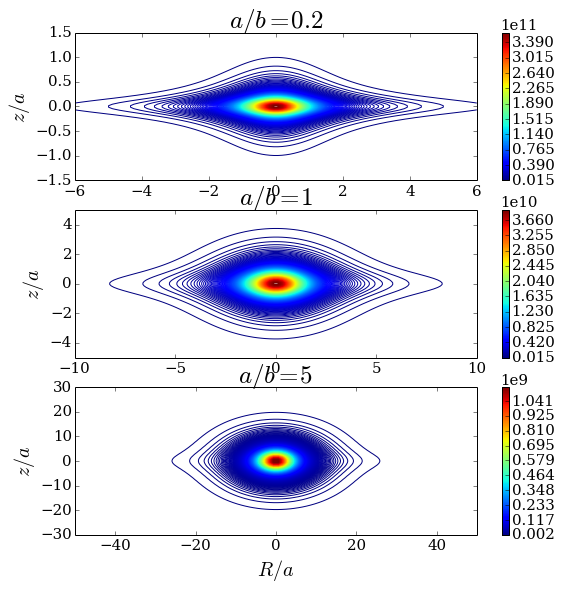
\includegraphics[scale=0.7]{MN_density_contours.png}
\end{figure}

\section{Logarithmic Profile}\label{sec:log}

Disc profile

\begin{equation}
\Phi_L(R, z) = \dfrac{1}{2} v_0^2 ln \left( R_c^2 + R^2 + \dfrac{z^2}{q_{\phi}^2}  \right) + constant
\end{equation}

The circular velocity at $z=0$ is $v_c^22(R, z=0) = r \dfrac{d \Phi}{dR}$:

\begin{equation}
v_c(R, z=0) = r \dfrac{d \Phi_L}{dr} = \dfrac{v_0 R}{\sqrt{r_c^2 + R^2}}
\end{equation}

\begin{figure}[H]
\centering
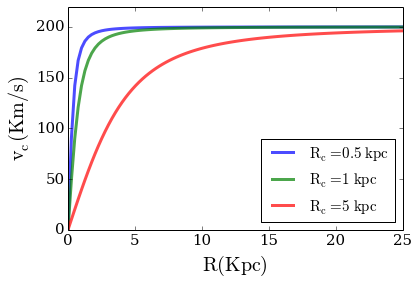
\includegraphics[scale=0.7]{Log_vc.png}
\end{figure}


To derive the density we make use of Poisson's equation in cylindrical coordinates:

\begin{equation}
\rho_L(R, z) = \dfrac{\nabla^2 \Phi_L}{4 \pi G } = \dfrac{1}{4 \pi G} \left( \dfrac{1}{r}\dfrac{d}{dR}R\dfrac{d}{dR}  + \dfrac{d^2}{dz^2}  \right) \Phi_L
\end{equation}

\begin{equation}
\rho_L(R, z) = \dfrac{v_0^2}{8 \pi G } \left( \dfrac{1}{R} \dfrac{4R ( R_c^2 + R^2 + \dfrac{z^2}{q_{\phi}^2} ) - 4R^3}{( R_c^2 + R^2 + \dfrac{z^2}{q_{\phi}^2} )^2} + \dfrac{\dfrac{2}{q_{\phi}^2} ( R_c^2 + R^2 + \dfrac{z^2}{q_{\phi}^2} ) - \dfrac{4z^2}{q_{\phi}^4}}{( R_c^2 + R^2 + \dfrac{z^2}{q_{\phi}^2} )^2}  \right)
\end{equation}

\begin{equation}
\rho_L(R, z) =  \dfrac{v_0^2}{4 \pi G q_{\phi}^2} \dfrac{(2q_{\phi}^2 + 1)R_c^2 + r^2 + (2 - q_{\Phi^2})z^2}{(R_c^2 + r^2 + z^2q_{\Phi}^{-2})^2}
\end{equation}


\begin{figure}[H]
\centering
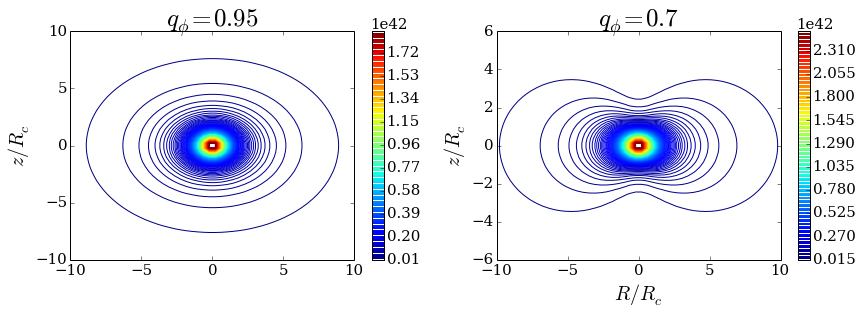
\includegraphics[scale=0.6]{MN_logarithmic_contours.png}
\end{figure}


\section{Logarithmic profile (Law, Johnston \& Majewski)}\label{sec:LJM05}

This profile is almost the same that the one explained in the previous section \ref{sec:log}

\begin{equation}
\Phi = v^2_{halo} ln[r^2 + (z^2/q^2) + d^2]
\end{equation}

\begin{equation}
v_c = \dfrac{\sqrt{2}vr}{\sqrt{r^2 + d^2}}
\end{equation}

with $q=0.8-1.45$, $v_{halo}$ should match $v_{circ, \odot}$, $d=1-20kpc$




\section{Logarithmic (Law \& Majewski 2010)}\label{sec:LM10}
\verb+http://iopscience.iop.org/0004-637X/714/1/229/pdf/apj_714_1_229.pdf+

\begin{equation}
\Phi = v^2_{halo} ln(C_1 x^2 + C_2y^2 + C_3 xy + (z/q_z)^2 r_{halo}^2)
\end{equation}

$R, r$ (Cylindrical, spherical)

\begin{equation}
C_1 = \left( \dfrac{cos^2 \phi}{q_1^2} + \dfrac{sin^2 \phi}{q_2^2}   \right)
\end{equation}

\begin{equation}
C_2 = \left( \dfrac{cos^2 \phi}{q_2^2} + \dfrac{sin^2 \phi}{q_1^2} \right)
\end{equation}

\begin{equation}
C_3 = 2 sin \phi cos\phi \left( \dfrac{1}{q_1^2} - \dfrac{1}{q_2^2} \right)
\end{equation}

\section{Modelling the MW}

\begin{table}[H]
%\begin{center}
\begin{scriptsize}
\begin{tabular}{c c c c c }
\hline 
Component  &  Besla07 &  LM2010 & Roeland12 & Gomez15 \\
\hline
Disk Model & Miyamoto-Nagai   & Miyamoto-Nagai &  &  \\
Disk Mass($M_{\odot}$) & $5.5^{10}$  & $1.0 \times 10^{11}$ & & \\
Disk Param & $R_d = 3.5$, $z=r_{disk}/5.0$  & $\alpha=1$ & &, $a=6.5kpc$, $b=0.26Kpc$\\
Bulge Model & Hernquist & Hernquist &  & Hernquist\\
Bulge Mass($M_{\odot}$) & $10^{10}$  &$3.4 \times 10^{10}$ & & \\
Bulge Param & $0.6 kpc$ &  $3.4 \times 10^{10}M_{\odot}$, $c=0.7kpc$   &0.6Kpc &\\
DM halo Model & NFW  & \ref{sec:LM10}  & Hernquist(NFW) & \\
DM halo mass($M_{\odot}$) & $10^{12}$ &$ \times 10^{10}$ & & \\
Halo Param & $c=11, r_{vir} = 258Kpc$& $r_{halo} = 12 Kpc$ & &\\
Solar distance $R_{\odot}$ (kpc) & 8.0 &   & & \\
reference &\href{http://adsabs.harvard.edu/abs/2007ApJ...668..949B}{Besla07} & \href{http://bit.ly/1fXtla9}{LM2010} & &  \\
\hline
\end{tabular}
\end{scriptsize}
%\end{center}
\end{table}




\begin{figure}[H]\label{MWBesla07}
\centering
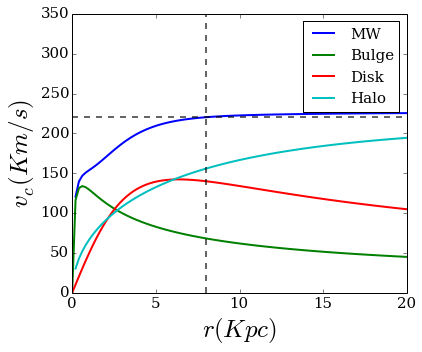
\includegraphics[scale=0.7]{MWBEsla07.png}
\end{figure}

\section{TO-DO:}

\begin{itemize}

\item Study the properties and different parameters ($M, /pho, v_c, a$)
\item Put all the plots and explnations in the text
\item note: Klypin relation between $c$ and $M_{vir}$ Doesn't take into 
account adiabatic contraction. 

\item work in the code that integrates the orbits using the accelerations. (Viernes)

\end{itemize}

\bibliographystyle{plain}
\bibliography{referencesDMMW}


\end{document}
